\chapter{Exciton polariton in complex lattices}\label{CHTHREE}
In this chapter, we consider the lattice with more than one site per unit cell which supports more than one band in the tight-binding model.

In the first part of the chapter, we study the formation of the compact localized state in exciton-polaritons condensation. Considering the Lieb lattice, we appliy a resonant Laguerre--Gaussian pulse to excite the condensate in the compact localized state and checked the evolution of the state with and without a background homogeneous incoherent pumping.
%In the first part of chapter, we show the excitation of a compact localized state of exciton-polaritons in a Lieb lattice by using resonant Laguerre--Gaussian pulses, and check the evolution of the excited state.

In the second part of the chapter, we considered the topological properties in exciton-polariton lattice system. We showed that by arranging local magnetic quantum dots (QDs) into a graphene pattern and considering TE-TM splitting, a non-trivial topological edge state can be found.
Further, by changing the magnitude of the local magnetic field, we found that the Chern number can change from $\pm 2$ to $\mp 1$.

\section{Excitation of localized condensates in the flat band of exciton-polariton Lieb lattice}\label{Ch4}
% %
% % ----------------------------------------------
% %
%\subsection{Flat bands in exciton-polaritons}
The full quench of single-particle kinetic energy is the main feature of dispersionless or flat bands (FBs)~\cite{Derzhko:2015aa,Leykam:2018aa,Leykam:2018ab}.
In many-body physics, even weak interations between particles become important in FB systems.
One example of interesting fermionic correlations is the fractional quantum Hall effect that appears in flat Landau levels.
Particles with bosonic statistics are also expected to dramatically change their properties under FB settings.
Due to the high degeneracy of the FB energy level, one can construct compact localized states (CLSs) that extend over a few lattice sites only for a specific tight-binding model.
The first such observation in a 2D dice lattice was found by Sutherland~\cite{Sutherland:1986aa}.
At a low concentration of bosonic particles, they can be distributed over several CLSs in such a way that their wave functions do not overlap, so that the total energy is minimized in the case of repulsive interaction between particles.
Thus, depending on the number of occupied sites, the bosons can develop a supersolid phase that features periodic density modulation~\cite{Huber:2010aa}.

This chapter applies an exciton-polariton approach to address the loading of bosons of finite lifetime into a FB and the related effects.
The exciton-polaritons represent strongly coupled states of microcavity photons and semiconductor QW excitons~\cite{Kavokin:2017aa}.
Driven-dissipative condensates of exciton-polaritons have been reliably observed in semiconductor microcavities~\cite{Kasprzak:2006aa,Balili:2007aa}; following this,
the potential of polariton condensates in artificial lattices for both applied and fundamental research has been well studied.
Examples include $\pi$-condensates at the edges of bands in 1D periodic potentials~\cite{Lai:2007aa}, and $d$-condensates in 2D square lattices~\cite{Kim:2011aa}.
Various methods of polariton trapping have been employed.
In particular, polariton condensates subject to spatially periodic acoustic phonon fields have been successfully created and studied~\cite{Cerda-Mendez:2010aa,Cerda-Mendez:2013aa}.
It was also shown that the periodic long-range order in a polariton condensate under resonant excitation can appear spontaneously~\cite{Gavrilov:2018aa}.

Interest has blossomed in exciton-polariton condensation in more complicated artificial periodic potentials, which target topologically protected~\cite{Karzig:2015aa,Nalitov:2015aa,Bardyn:2015aa,St-Jean:2017aa,Li:2018aa,Solnyshkov:2018aa} and single-particle FBs.
Such condensation has been studied in honeycomb~\cite{Jacqmin:2014aa}, kagome~\cite{Masumoto:2012aa,Gulevich:2016aa}, 1D Lieb~\cite{Baboux:2016aa} and 2D Lieb~\cite{Klembt:2017aa,Whittaker:2018ab} lattices.
In FB systems, the coherence length of polariton condensates only extends to a small number of lattice sites; two possible explanations for this are that the potential disorder limits the range or more simply that the fragmentation is a generic feature of non-equilibrium condensation in FBs.

The lattice considered here is a 2D Lieb lattice with a geometry similar to the one in~\cite{Klembt:2017aa}.
We investigate the combined effect of distributed dissipation and exciton-photon coupling on the band structure.
In the following sections, by examining both the energy and lifetime of the particles, we identify possible candidate states for condensation in each band. We show that while no perfect FB exists in this continuous, ``non-tight-binding'' system, the concept of long-lived strongly localized states, as maintained by the destructive interference of propagating waves, is still valid to some degree.

%
% ---------------------------------------
%
\subsection{2D Lieb lattice and band structure}
%
%
%
\begin{figure}[ht]
\centering
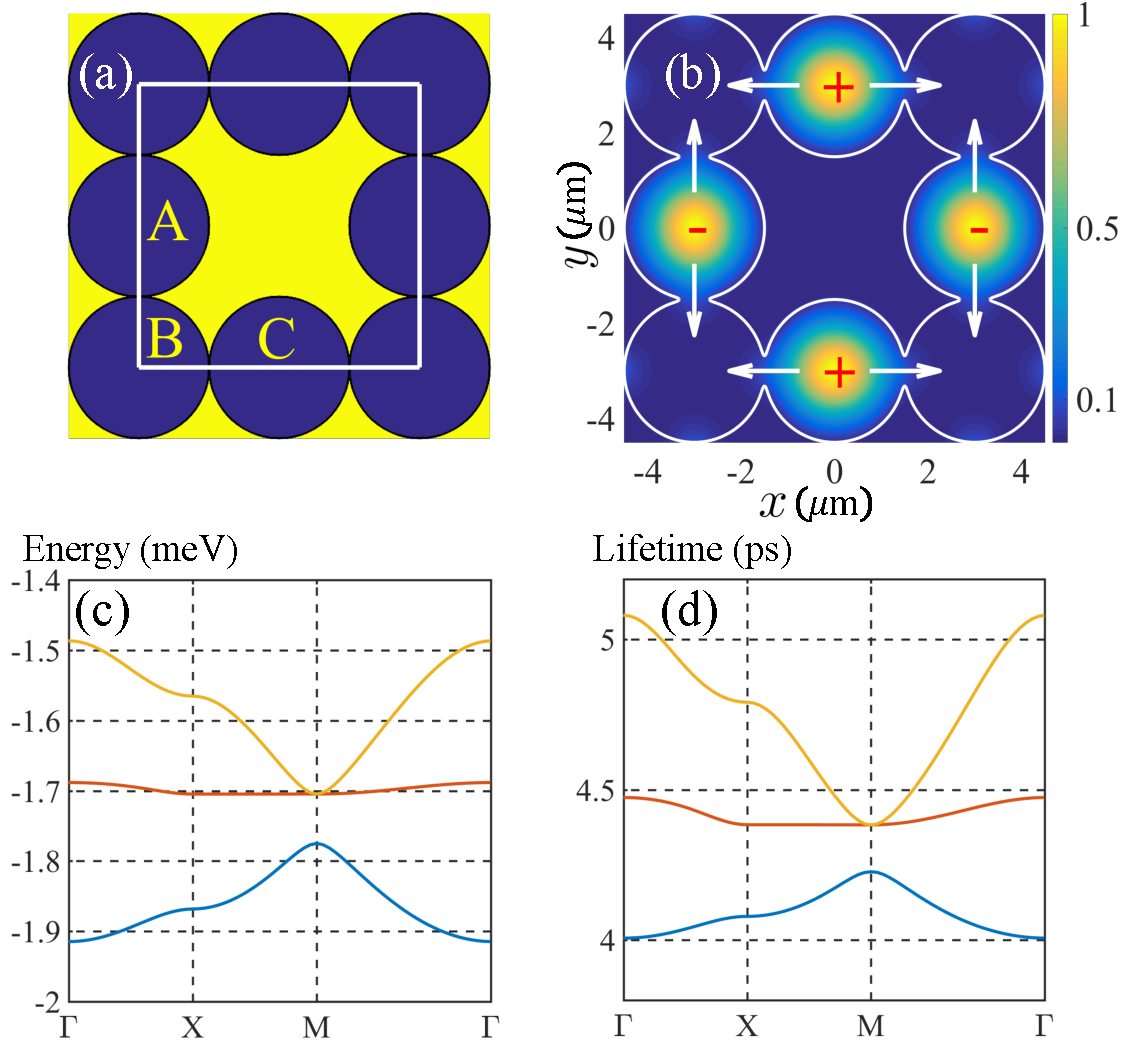
\includegraphics[width=0.6\linewidth]{Fig/Ch3/pic1.pdf}
\caption[Lieb lattice and corresponding spectrum]{(a,b) System schematics and (c,d) single-particle spectra.
(a) The Lieb lattice plaquette including three pillars (QWs) per unit cell: A, B, and C.
(b) Probability density of the photonic component of the single-polariton (Bloch) state of the nearly flat (second) band at the $\Gamma$-point.
Signs indicate the wave function phase. The weak population of the B sites is not visible.
A CLS possesses a similar structure and will not propagate along the arrow directions due to destructive interference caused by the $\pi$-phase difference at sites A and C.
(c) The real part of the energy of the single-particle Bloch bands.
(d) The lifetimes of the Bloch states (the inverse imaginary part of the eigenvalues).
 The figure is taken from~\cite{Sun:2018aa}.}
\label{fig:CH3_1}
\end{figure}
%
%
%
The exciton-polariton condensate wave function can be written as $\Psi=(\varphi,\chi)^\mathrm{T}$, where $\varphi$ and $\chi$ are the photonic and excitonic components, respectively.
The mean-field Hamiltonian of the system reads (we set $\hbar=1$)
%
\begin{equation}
  \hat{H} =
  \begin{pmatrix}
  -\frac{\nabla^2}{2m_c}+V(\mathbf{r}) & \Omega \\
  \Omega & \delta -\frac{\mi}{2\tau_x} -\frac{\nabla^2}{2m_x}+\alpha_x|\chi|^2
  \end{pmatrix},
  \label{CH3_Ham}
\end{equation}
where $m_c$ and $m_x$ are the microcavity photon and exciton effective masses, respectively, $\Omega$ is the Rabi frequency, $\alpha_x$ is the exciton--exciton interaction strength, $\tau_x$ is the exciton lifetime, and $V(\mathbf{r})=V_r(\mathbf{r})-{\mi}V_i(\mathbf{r})$ is the complex-valued potential experienced by the photonic component separately from the excitonic component~\cite{Sun:2017ab}.
The real part of the potential $V_r$ is defined by the QWs that form the Lieb lattice [see Fig.~\ref{fig:CH3_1}(a)]. The imaginary part $V_i$ describes the distributed losses in the system.
We set $V_r=0$ and $V_i=0.1\,\mathrm{meV}$ inside the wells, while  $V_r=30\,\mathrm{meV}$ and $V_i=2.1\,\mathrm{meV}$ in the barriers.
It should be noted that photon lifetime is expected to be nonuniform; indeed, the barriers are usually produced by a partial etching of the DBRs, which introduces additional photon leakage from the barrier area.
The diameter of each QW is $3\,\mu\mathrm{m}$ and the lattice constant is $a=6\,\mu\mathrm{m}$.
The other parameters are $\hbar\Omega=4.25\,\mathrm{meV}$, $m_c=3.2\times10^{-5}\,m_e$, $m_x=10^5\,m_c$, $\tau_x=100$ ps, and the detuning is $\delta=-4.0\,\mathrm{meV}$.
Here, $\tau_x^{-1}\ll-2\mathrm{Im}\{V(\mathbf{r})\}$, so that the losses in the polariton system are controlled by the photonic component.

The unit cell of the Lieb lattice is composed of three QWs labeled A, B, and C, as shown in Fig.~\ref{fig:CH3_1}(a).
It is well known that in the framework of a tight-binding model the system spectrum possesses a FB.
The CLS in the tight-binding FB is located on the A and C sites of a single .
The phases on A and C are shifted by $\pi$, and the CLS is maintained due to the destructive interference of waves propagating from A and C sites to B~\cite{Vicencio:2015aa}.
The Bloch state of the second (nearly) FB at the $\Gamma$-point, as shown in Fig.\ref{fig:CH3_1}(b), has a similar structure except that it extends over the whole lattice.
This state also shows a $\pi$ phase shift between A and C sites, in addition to a very weak excitation of the B sites.

Figure~\ref{fig:CH3_1}(c) shows the three lowest bands representing the spectrum of noninteracting polaritons ($\alpha_x=0$).
It is clear that the continuous model [Eq.~\eqref{CH3_Ham}] does not lead to a perfect FB.
The middle band, which is flat within the tight-binding model with nearest-neighbor hopping, shows a small but finite dispersion.

Another key feature of this system concerns the dispersion of losses in the bands, as shown in Fig.~\ref{fig:CH3_1}(d).
For the lowest band, the state with the smallest losses occurs at the corner of the Brillouin zone (M point) with the wave vector $k_x={\pm}k_y={\pm}\pi/a$.
For the middle (nearly flat) band, minimum dissipation takes place at $k=0$ ($\Gamma$ point).
The wave function of this state corresponds to highly occupied A and C sites and nearly empty B sites, as shown in Fig.~\ref{fig:CH3_1}(b).

%
% -------------------------------------
%
\subsection{Laguerre--Gaussian resonant pumping}
We excite the compact localized condensate (CLC) of the middle band in Fig.~\ref{fig:CH3_1}(c), i.e. the FB, by exposing the Lieb lattice structure to a short resonant (ring-shaped) Laguerre--Gaussian pulse centered at one.
The polariton wave function in this case evolves according to
%
\begin{equation}\label{CH3_Evol}
  \mi\dot{\Psi} = \hat{H}\Psi+\begin{pmatrix} \mi P(\mathbf{r},t)\\{0}\end{pmatrix},
\end{equation}
%
where the pulse profile is given by~\cite{Kim:1999aa}
%
\begin{equation}\label{CH3_Pulse}
  P(\mathbf{r},t)=P_0 \frac{(x\pm{\mi}y)^2}{R^2}
  \exp\!\left[-\frac{r^2}{R^2}-\mi\omega_0t\right]\!\theta(t)\theta(t_p-t).
\end{equation}
%
Here, $P_0$ is the pulse amplitude, $R$ is the  radius of the pulse ring, $\omega_0$ is the frequency of the pulse coinciding with the frequency of the FB at the $\Gamma$ point, $\theta(t)$ is the Heaviside step function, and $t_p$ is the pulse duration.
Transport of polaritons to the B sites should be blocked due to the $\pi$-phase difference of the wave functions on the A and C sites.
The phase and intensity plot in Fig.~\ref{fig:CH3_2}(a) shows that we can achieve this $\pi$ phase difference by centering the pump beam at the center of the unit cell.

%
% ---------------------------------------
%
\subsection{Dynamics of the CLC}
To characterize the CLC dynamics, it is convenient to use the function
%
\begin{equation}\label{CH3_NCLS}
N_\textrm{CLS}\left(t\right)=N_c(t)+N_x(t)=\int_{\textrm{A,C}}\left(|\varphi|^2+|\chi|^2\right) d^2r
\end{equation}
%
that measures the total number of particles residing at the A and C sites of the excited plaquette.
We trace the evolution of the system just after the pulse is switched off at $t=0$.
Figure~\ref{fig:CH3_2}(b) shows the particle decay rate in the CLC for different intensities of interaction strength and coherent pumping.

A counterintuitive result in Fig.~\ref{fig:CH3_2}(b) is a decrease of particle loss from CLC with increasing polariton--polariton interaction strength $\alpha_x$, or alternatively, with increasing the coherent pumping amplitude $P_0$, which increases the number of particles in the condensate and elevates the role of interaction.
Despite the repulsive nature of exciton--exciton interaction, as the figure shows it has a focusing effect on the CLC in the Lieb lattice.

Other than a gradual decay of the excited CLC, we observe fast Rabi oscillations of particle number and more complex short and long-time dynamics.
To highlight these effects arising from the two-component (exciton and photon) nature of polaritons and their continuous, ``non-tight-binding'' propagation, we also consider CLC dynamics in the absence of dissipation.
Figure~\ref{fig:CH3_2}(c) and (d) show snapshots of the particle density $\left(|\varphi(\mathbf{r},t)|^2+|\chi(\mathbf{r},t)|^2\right)d^2r$ at $t=1.6\,\mathrm{ps}$ and $t=30\,\mathrm{ps}$, respectively.
Due to the shape of the Laguerre--Gaussian pulse, the condensates excited in the A and C wells are smaller than the well size.
%These condensates bounce against the QW boundaries with a period of $\sim 2\,\mathrm{ps}$, see Supplemental Materials (videos of this motion).
%
%
%
\begin{figure}[ht]
\centering
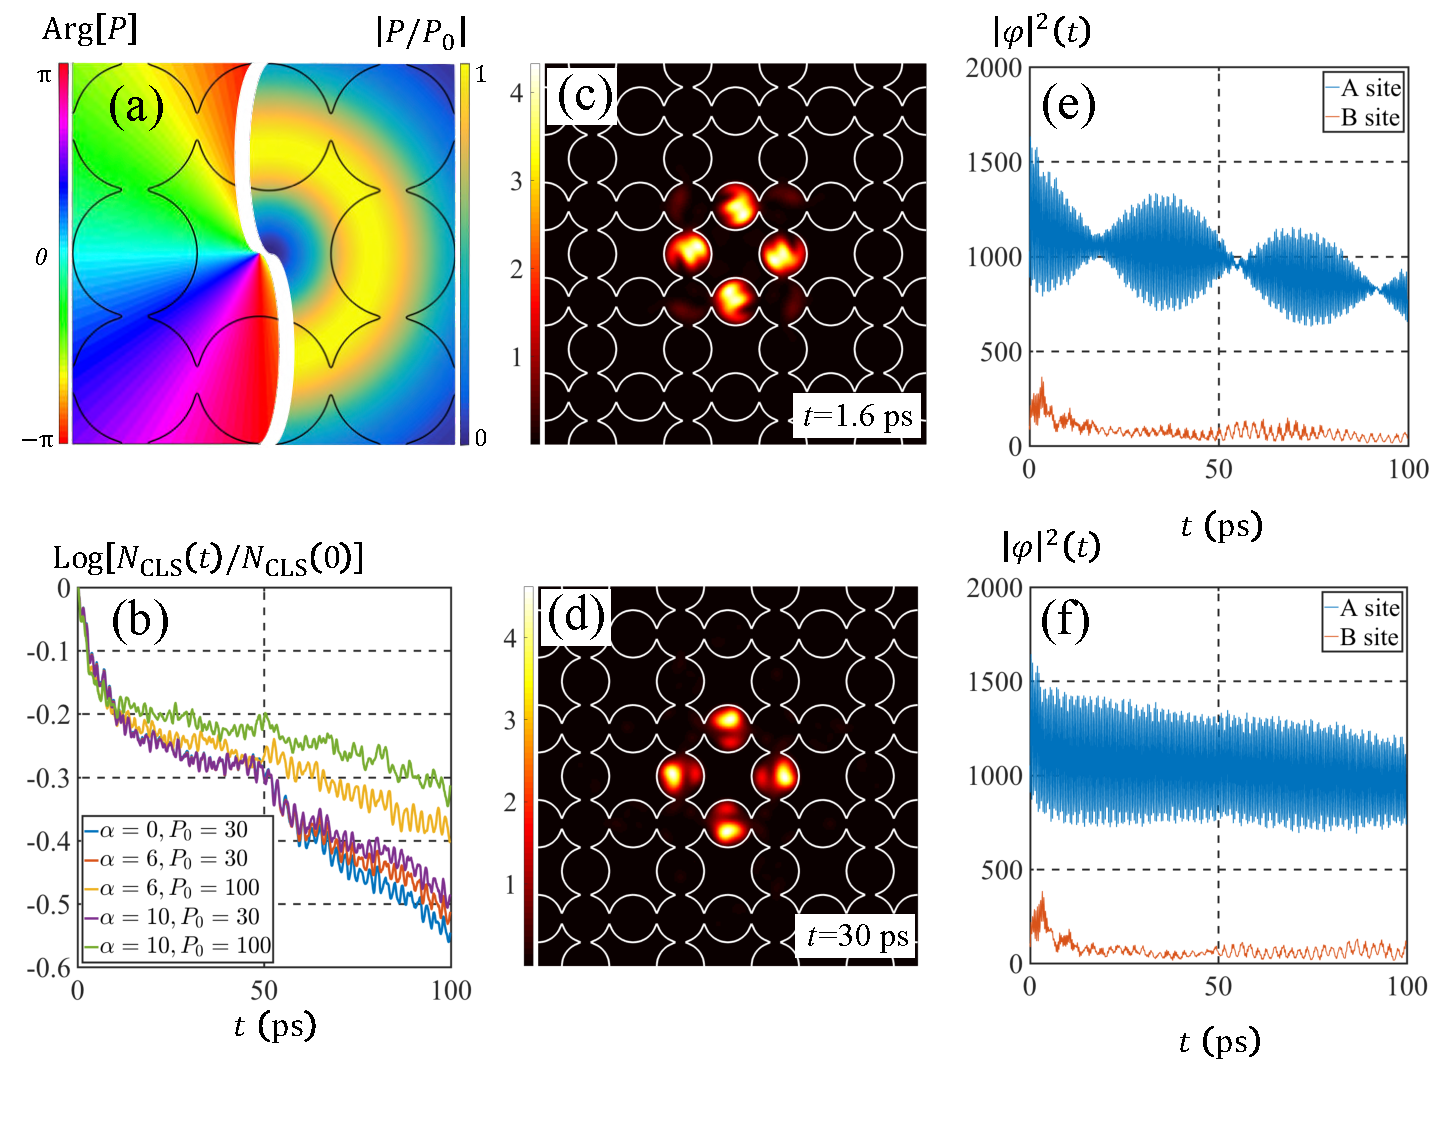
\includegraphics[width=0.79\linewidth]{Fig/Ch3/pic2.pdf}
    \caption[Laguerre--Gaussian pulse and corresponding CLC dynamics]{(a) Phase and intensity of the Laguerre--Gaussian pulse with a radius of $R=1.5\,\mu$m centered at the Lieb lattice plaquette. (b) Decay of the CLC for different magnitudes of the interaction strengths $\alpha_x$ in units of $\mu\mathrm{eV}\cdot\mu\mathrm{m}^2$ and the coherent strength $P_0$ in units of $\mathrm{meV}\cdot\mu\mathrm{m}^{-1}$.
(c--f) Dynamics of the CLC in the absence of dissipation.
(c,d) Snapshots of CLC particle density distribution $\left(|\varphi(\mathbf{r},t)|^2+|\chi(\mathbf{r},t)|^2\right)d^2r$
at two different times for $\alpha_x=10\,\mu\mathrm{eV}\cdot\mu\mathrm{m}^2$.
(e,f) Rabi oscillations of the photonic component from the A and B sites for $\alpha_x=0$ (e) and $\alpha_x=10\,\mu\mathrm{eV}\cdot\mu\mathrm{m}^2$ (f) with $P_0=100\,\mathrm{meV}\cdot\mu\mathrm{m}^{-1}$. The figure is taken from~\cite{Sun:2018aa}.
}
\label{fig:CH3_2}
\end{figure}
%
%
%

We can also see a slow modulation of the amplitude of the Rabi oscillations of the photonic component, which can be measured experimentally~\cite{Dominici:2014aa}.
Figure~\ref{fig:CH3_2}(e) and (f) show the time dependence of the total number of photons in an A site (the same as in a C site), as well as in a B site.
For the interaction-free case [Fig.~\ref{fig:CH3_2}(e)], one can see that the condensate dynamics at the A and C sites is characterized by fast Rabi oscillations with a slow beating of their amplitude.
The beating half-period $t_b$ is about $30\,\mathrm{ps}$; this matches the width of the FB ${\Delta}E_f\simeq0.02\mathrm{meV}\simeq\hbar/t_b$, and thus the effect likely results from the finite band width.
In the presence of polariton--polariton interaction, the beatings of the Rabi oscillations on the A(C) sites are smoothed out [Fig.~\ref{fig:CH3_2}(f)]. Note that occupation in the B sites is very low in both cases.

%
% --------------------------------------
%
\subsection{Prolonging the CLC}
Polariton lifetime in etched microcavities is typically short, which makes it hard to maintain and manipulate condensates for times longer than several ps.
It follows from Fig.~\ref{fig:CH3_2}(d) that the lifetime of particles in the CLS (second band at the $\Gamma$ point) is $\tau_\textrm{CLS}\approx4.5$ ps.
One way to increase the lifetime would be to use microcavities with higher Q factors; alternatively, losses can also be compensated for by incoherent background pumping to maintain the CLC
When incoherent background pumping is present, the evolution of the system is described by the equations
%
\begin{subequations}\label{CH3_INC}
\begin{align}
 \mi\begin{pmatrix}\dot{\varphi}\\\dot{\chi}\end{pmatrix} &=
 \hat{H}\begin{pmatrix}{\varphi}\\{\chi}\end{pmatrix}
 +\frac{{\mi}cn_r}{2}\begin{pmatrix}{0}\\{\chi}\end{pmatrix}
 +\begin{pmatrix}{\mi P(\mathbf{r},t)}\\{0}\end{pmatrix}, \\[5pt]
 \dot{n}_r &= I - \tau_r^{-1} n_r-c|\chi|^2n_r,
\end{align}
\end{subequations}
%
where $n_r$ is the density of the reservoir particles, $\tau_r=10\,\mathrm{ps}$ is their lifetime, $c=0.005$ ps$^{-1}\mu$m$^2$ is a phenomenological reservoir-system coupling rate, and $I$ is the intensity of the homogeneous incoherent pumping.
The reservoir dissipation rate $\tau_r^{-1}$ is considered to be of the same order of magnitude as the polariton dissipation rate $-2\mathrm{Im}\{V(\mathbf{r})\}$, which is usually assumed for polariton systems under non-resonant pumping~\cite{Ostrovskaya:2012aa,Ma:2016aa} including polariton lattices~\cite{Ma:2015aa,Yulin:2016aa}.%\footnote{See also Refs.~\cite{Borgh:2010aa,Liew:2015aa} for the alternative approach, which assumes the reservoir rate to be much larger than the polariton one, allowing adiabatic exclusion of the reservoir}.
To avoid polariton excitation in the first and third (and higher) bands, we consider intensity $I$ to be below the polariton condensation threshold.
Below, we use the following threshold intensity $I_{th}=(c\tau_r \tau_x)^{-1}$ as a reference.
%
%
%
\begin{figure}[ht]
\centering
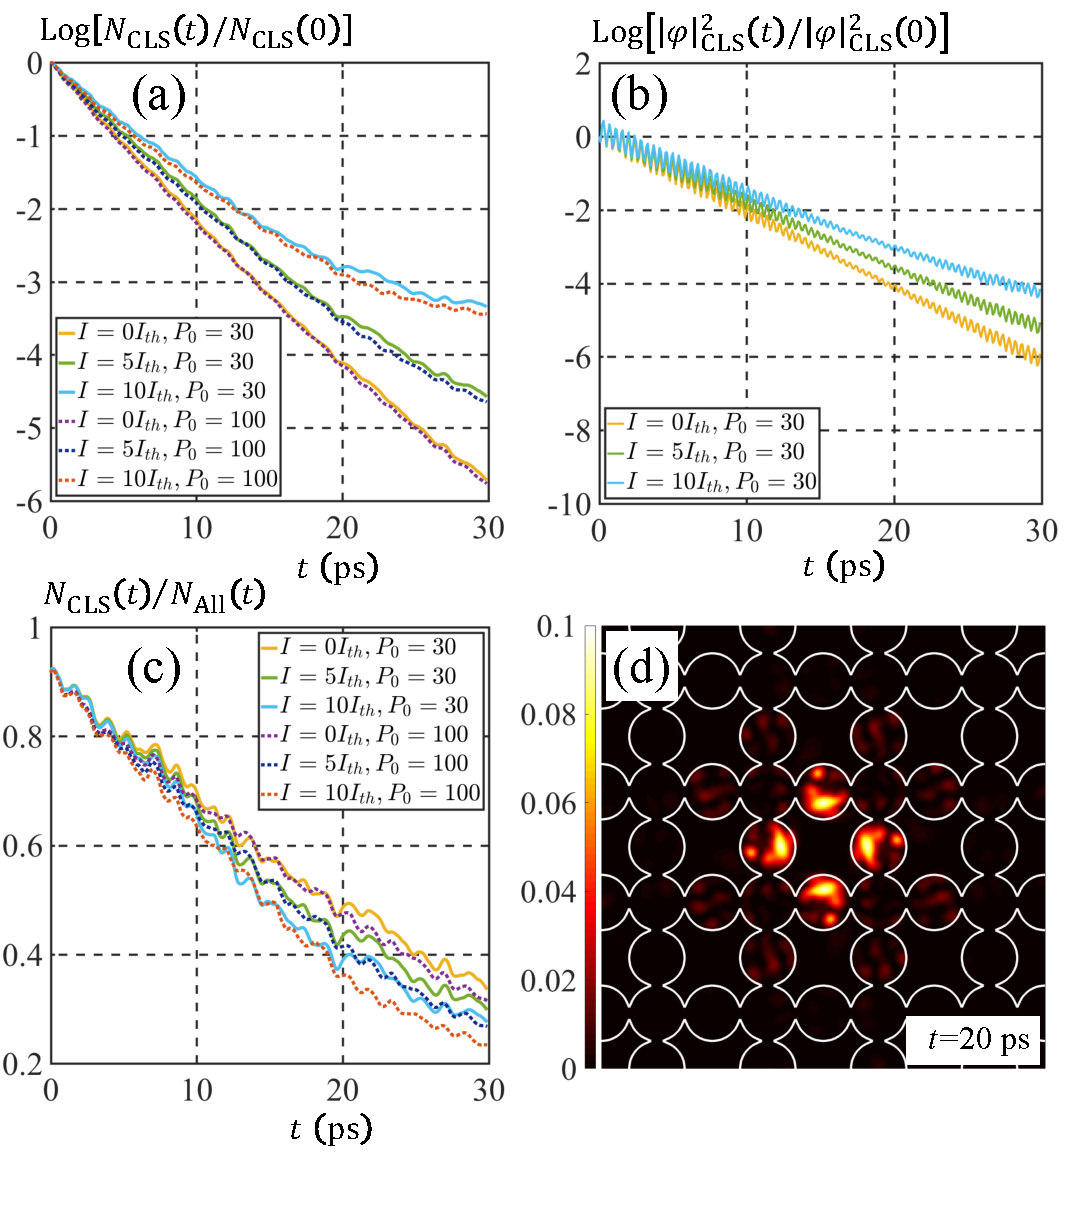
\includegraphics[width=0.55\linewidth]{Fig/Ch3/pic3.pdf}
\caption[CLC with incoherent pumping]{(a) Decay of the CLC for different incoherent pumping intensities $I$ (and various coherent pumpings $P_0$). The Laguerre--Gaussian resonant pulse radius is $R=1.5~\mu$m. (b) Photonic decay of the CLC for different incoherent pumping intensities. (c) Evolution of the ratio of CLC particles and the total number of particles for different incoherent pumping intensities. (d) Snapshot of the particle density in the CLC at 20~ps. The figure is taken from~\cite{Sun:2018aa}.}
\label{fig:CH3_3}
\end{figure}
%
%
%

Figure~\ref{fig:CH3_3}(a) shows the decay of particles residing in the CLC for different pumping intensities (both incoherent and coherent) together with a reference curve of the decay at $I=0$.
The increase of $I$ compensates for the decay of particles from the CLC.
The corresponding photonic decay also shows a similar behavior, as seen in Fig.~\ref{fig:CH3_3}(b).
One can see from both panels that the Rabi oscillations persist in the presence of incoherent background pumping, indicating that the CLC maintains its coherence.

Several drawbacks accompany the use of incoherent pumping.
First, it leads to the excitation of particles in other (non-flat) bands and thus increases the occupation of the B sites. Second, although background pumping preserves the CLC for longer times, it also generates noise.
Figure~\ref{fig:CH3_3}(c) shows the ratio of particles in the CLC to the total number of particles in the system: the larger the $I$, the worse the signal-to-noise ratio.
At $I=10I_\mathrm{th}$ and after 20~ps, about $60\%$ of the polaritons already escaped from the CLC.
Despite this, the four CLC QWs containing only $40\%$ of the polaritons remain the most populated wells, as shown in Fig.~\ref{fig:CH3_3}(d).
We can conclude then that the background pumping prolongs the CLC for one order of magnitude longer times than single-polariton lifetimes.

%
% ------------------------------------------
%
\subsection{Discussion}
Using an example of a realistic 2D exciton-polariton Lieb lattice with distributed losses, we have shown that the (nearly) flat band in this system possesses small but finite dispersion, both in the energy and the lifetime of the states.
We have demonstrated the possibility to excite compact localized condensates in this nearly FB using resonant Laguerre--Gaussian pulses.
In spite of the small dispersion of the band, the localization and coherence of the compact localized condensates remain well defined.
They exhibit unusual dynamics, following from modulated fast Rabi oscillations.
This coherent excitation of CLCs opens new possibilities to use polariton Lieb lattices as platforms for network computations; in particular, it permits to construct CLC graphs, similar to recent proposals for classical~\cite{Berloff:2017aa,Ohadi:2017aa} and quantum~\cite{Liew:2018aa} simulators.
In the presence of an incoherent homogeneous background pumping, the coherent compact localized condensates can be maintained for times much longer than regular polariton lifetimes.
Thus, both the phase and polarization of localized condensates may be able to be used to encode information in the future.
%The main benefits of the FB states in the Lieb lattice consist of their compactness and suppressed in-plane spreading, as well as better control of multiple CLC arrangements, where the underlying Lieb structure sets all distances between CLCs.
